\documentclass{../template/myrpt}
\ExamName{稳压电路的特性与设计}

\newcolumntype{Y}{>{\centering\arraybackslash}X}
\newcolumntype{C}[1]{>{\centering\arraybackslash}m{#1}}
\newcommand{\blankcell}{\rule{0pt}{1.15cm}}

\begin{document}
\maketitle

\section{实验目的}
\begin{enumerate}[label=\arabic*. ]
  \item 掌握稳压电路的工作原理及各元件在电路中的作用；
  \item 学习直流稳压电源的安装、调试和测试方法；
  \item 熟悉线性集成稳压电路的工作原理；
  \item 学习线性集成稳压电路主要技术指标的测量方法。
\end{enumerate}

\section{实验仪器}

9 孔插件板、交流电源、数字万用表、电容器（$0.1\,\si{\micro\farad}$、$1\,\si{\micro\farad}$、$470\,\si{\micro\farad}$）、电阻（$100\,\si{\ohm}$、$200\,\si{\ohm}$、$1\,\si{k\ohm}$）、$10\,\si{k\ohm}$ 电位器、二极管、三端稳压器 7805、双踪示波器及连接线。

\begin{figure}[htbp]
  \centering
  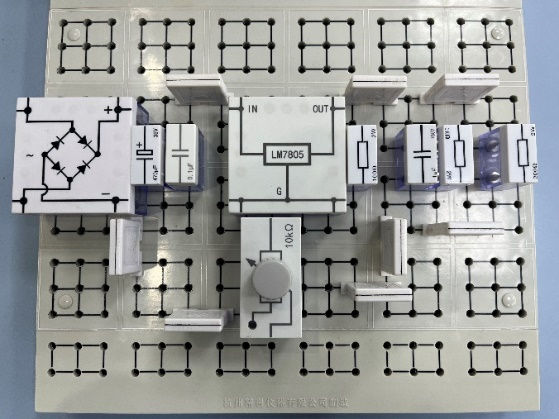
\includegraphics[width=0.78\linewidth]{assets/media/apparatus.jpeg}
  \caption{9 孔插件板及稳压电路实验装置}
  \label{fig:apparatus}
\end{figure}

\section{实验原理}

\subsection{直流稳压电源的组成}

当输入电压、负载或环境条件发生变化时，仍能使输出电压保持相对稳定的电路称为稳压电路。直流稳压电源通常由变压、整流、滤波和稳压四部分组成，其基本框图如图~\ref{fig:block} 所示。本实验主要研究由线性集成稳压器 7805 构成的稳压电路。

\begin{figure}[htbp]
  \centering
  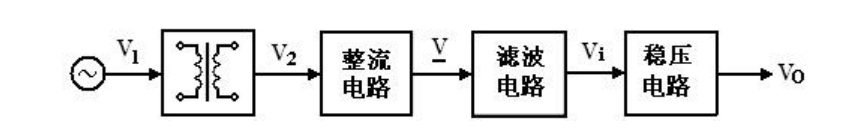
\includegraphics[width=0.88\linewidth]{assets/media/block-diagram.png}
  \caption{直流稳压电源框图}
  \label{fig:block}
\end{figure}

固定输出为 $5\,\si{\volt}$ 的电路如图~\ref{fig:fixed} 所示；通过电位器 $R_W$ 调节取样电压，可获得可调输出稳压电路，如图~\ref{fig:adjustable} 所示。$C_1$ 为整流后的滤波电容，$C_2$ 用于抑制稳压器自激振荡，$C_3$ 用于旁路高频噪声。

\begin{figure}[htbp]
  \centering
  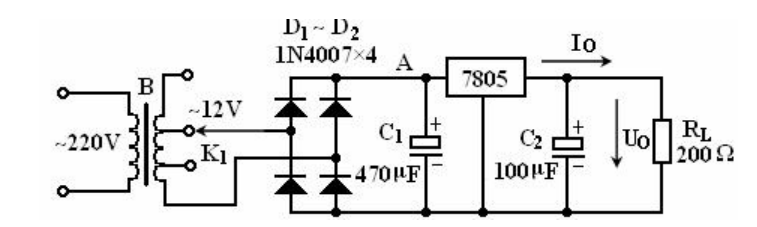
\includegraphics[width=0.92\linewidth]{assets/media/fixed-5v.png}
  \caption{固定输出为 $5\,\si{\volt}$ 的稳压电路}
  \label{fig:fixed}
\end{figure}

\begin{figure}[htbp]
  \centering
  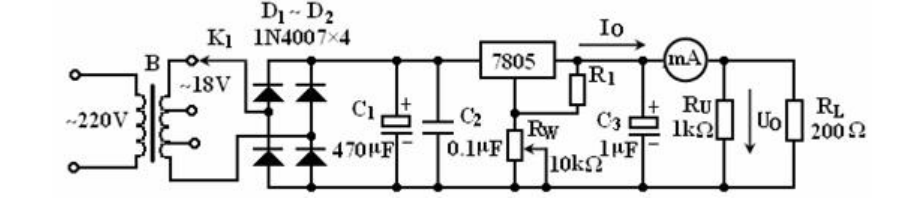
\includegraphics[width=0.96\linewidth]{assets/media/adjustable.png}
  \caption{可调输出稳压电路}
  \label{fig:adjustable}
\end{figure}

\subsection{主要技术指标}

稳压系数定义为负载电流和环境温度不变时，输出电压相对变化量与输入电压相对变化量之比：
\begin{equation}
  \label{eq:voltage-regulation}
  S_r=\frac{\Delta U_o/U_o}{\Delta U_i/U_i}.
\end{equation}
纹波抑制比定义为输入、输出纹波电压峰峰值之比的对数值：
\begin{equation}
  \label{eq:ripple-rejection}
  S_{S\mathrm{RPP}}=20\lg\frac{U_{i\mathrm{PP}}}{U_{o\mathrm{PP}}}.
\end{equation}
纹波抑制比越大，说明稳压电路抑制交流纹波的能力越强。

在输入电压不变时，输出电阻可由开路输出电压 $U'_o$ 和接入负载后的输出电压 $U_o$ 求得：
\begin{equation}
  \label{eq:output-resistance}
  R_o=\left(\frac{U'_o}{U_o}-1\right)R_L.
\end{equation}

交流电经变压后首先进入整流电路。桥式整流每半周期由两只二极管导通，使负载两端的电压始终保持同一极性，输出纹波频率因而约为电源频率的两倍。整流后的脉动电压经 $C_1$ 充放电：在波峰附近电容充电，在两个波峰之间向负载放电。电容越大，放电电压下降越慢，但上电流冲击和体积也会增大。

线性稳压器位于滤波级之后，主要消除滤波后仍然存在的低频纹波和输入电压缓慢变化。它并不是以降压电阻的方式被动工作，而是通过负反馈实时检测输出，主动改变串联调整元件的压降。当输入或负载变化使输出下降时，调整元件导通增强；当输出升高时，导通程度减小，从而使输出回到设定值附近。

7805 使用时需满足一定的输入输出压差，以保证内部调整管保持在可控工作区。输入过低时，调整管饱和，输出会跟随输入下降；输入过高时，多余电压主要落在调整管上并转化为热量。因此实验中应注意散热，避免长时间在大输入压差和大负载电流状态下运行。

可调输出电路中，$R_W$ 与固定电阻构成取样网络，滑片位置改变后，反馈端电压随之改变，因而输出可调。调节时不应一次旋转过大，而应在输出电压稳定后缓慢改变，同时观察波形是否出现振荡、失真或突然跳变。

稳压系数反映电网或前级电压变化时输出的敏感程度，数值越小表明输出越稳定。纹波抑制比用分贝表示输入与输出纹波幅度的比值，每增加 $20\,\si{\decibel}$ 意味着电压比缩小一百倍。输出电阻则用于衡量负载变化对输出电压的影响，是电源带负载能力的重要指标。

这三个指标分别对应输入稳定性、交流纹波抑制能力和负载稳定性。实际评价稳压电路时，应同时考察这些指标，不能只根据某一个输出电压读数判断电路性能。

在设计和调试稳压电源时，还需考虑稳压器的瞬态响应。当负载电流突然增大时，输出电压会先出现短时下跌，然后在反馈环路调节下恢复；当负载突然减小时，则可能出现短时上冲。输出电容 $C_3$ 可以改善高频瞬态，但电容过大也可能引起稳压器启动和关断时的反向放电问题。实际电路应按元件手册要求配置输入、输出旁路电容，并保证引线较短、接地良好。

稳压器的散热条件也是原理分析中不能忽略的因素。调整管消耗的功率近似为
\[
  P_D\approx(U_i-U_o)I_o.
\]
当输入电压较高、输出电流较大时，$P_D$ 增大，若结温升高会使基准电压和调整特性发生漂移，从而引起输出电压慢速变化。因此，输出范围测量应在温度相对稳定时进行，不宜在刚通电的瞬间记录极值。

从波形角度看，整流后波形的峰值、谷值和周期可以反映整流桥和滤波电容是否正常工作。波形局部出现振荡可能与探头接地回路过大、输出电容与稳压器不匹配或负载线路引入反馈有关。调试时应先分别观察输入、整流后和稳压后三个节点，再根据波形变化定位问题。
对于整流电路，电容滤波后的纹波电压还可用近似关系式估算：
\[
  U_{r\mathrm{PP}}\approx\frac{I_o}{f_r C},\qquad f_r=2f_{\text{网}}.
\]
该式表明，在负载电流增大时纹波增大，提高滤波电容或提高整流频率可减小纹波。但电容只能降低纹波，不能完全代替稳压器抵消输入电压的缓慢变化。
稳压器输出电压的瞬时变化可分为直流工作点变化和交流纹波两部分：
\[
  u_o(t)=U_{O}+u_{o\mathrm{r}}(t),
  \qquad \overline{u_{o\mathrm{r}}(t)}=0.
\]
其中 $U_O$ 是一个周期内的平均值，$u_{o\mathrm{r}}(t)$ 是变化的交流分量。测量时如果交流耦合、限带和探头接地设置不一致，屏幕上的峰峰值就不能直接代表纹波。

\clearpage

\section{实验内容和步骤}

\subsection{搭建并检查 7805 稳压电路}
按图~\ref{fig:adjustable} 在插件板上连接电路。接好后在 A 点断开，测量并记录输入电压 $U_i$（即 A 点电压）的波形；再接通 A 点后面的电路，观察输出电压 $U_o$ 波形并检查有无振荡。调节 $R_W$，若输出电压随之变化，则说明电路基本工作正常。
连接前先检查电源极性、二极管方向、电解电容正负极性以及 7805 的输入、接地和输出引脚，确认万用表处于直流电压档。通电后不要立即把 $R_W$ 旋到极限位置，应先在中间位置检查输出是否有稳定直流电压。若出现输出电压突然为零、电流异常增大或稳压器明显发热，应立即断电排查。
示波器测量时，探头地夹应接在电路公共地端，不能随意夹在整流桥任一浮空节点。先用较大的垂直量程找到波形，再逐步减小量程以提高读数分辨率；时基应选择使屏幕中包含多个周期，触发电平调到波形稳定为止。记录频率、峰峰值、有效值和波形特征，并注意区分交流耦合、直流分量和仪器噪声。

在开始正式记录前，应设置一个便于读数的测量档位，让波形占据屏幕高度的一半以上，并在同一配置下记录各项参数。对于自动测量结果，应检查测量窗口内是否包含整数个周期，否则周期、频率和峰峰值可能随采样窗口变化。记录时应保留原始单位，后续计算时再统一换算，避免把 \si{\milli\volt} 误记为 \si{\volt} 而产生千倍误差。

\subsection{测量输出电压范围}
调节 $R_W$，用示波器监视输出波形，分别测量稳压电路的最大、最小输出电压及相应输入电压，并测量稳压块基准电压（$100\,\si{\ohm}$ 电阻两端电压）。
测量输出范围时应缓慢旋转电位器，每次调节后等待稳定再读数。输出电压刚开始随 $R_W$ 近似线性变化，到达调节端点时可能出现不再上升或波形明显失真。记录最大和最小值时，应同时记录输入电压、基准电压和输出电压的状态，以便判断是调节范围受限还是稳压器已经退出稳压区。

\begin{LabRecordTable}
  \centering
  \caption{稳压电路输出范围}
  \label{table:output-range}
  \renewcommand{\arraystretch}{1.45}
  \small
  \begin{tabularx}{\textwidth}{C{5.0cm} Y}
    \toprule
    测量状态 & 输出电压 $U_o/\si{\volt}$ \\
    \midrule
    最大输出 & 14.41 \\
    最小输出 & 5.06 \\
    \bottomrule
  \end{tabularx}
\end{LabRecordTable}

\subsection{观察输入、输出纹波}
调节 $R_W$ 使 $U_o\approx5\,\si{\volt}$，分别用示波器观察稳压电路输入、输出电压波形，记录纹波电压峰峰值并进行比较。
纹波测量应固定输出工作点，使每次读数都在相同的输出电压附近完成。先观察整流滤波后的输入波形，再观察 7805 输出端波形，记录时基、垂直量程和交流耦合设置。对于幅度很小的输出纹波，应选择合适的带宽限制和平均模式，但不能把滤波后的噪声误当作纹波。若波形不稳定，应先调整触发源和探头接地，再进行峰峰值测量。

\begin{LabRecordTable}
  \centering
  \caption{输入、输出纹波电压测量}
  \label{table:ripple}
  \renewcommand{\arraystretch}{1.45}
  \small
  \begin{tabularx}{\textwidth}{C{5.0cm} Y Y}
    \toprule
    测量项目 & 输入纹波电压 $U_{i\mathrm{PP}}/\si{\volt}$ & 输出纹波电压 $U_{o\mathrm{PP}}/\si{\milli\volt}$ \\
    \midrule
    峰峰值 & 1.01 & 6.37 \\
    \bottomrule
  \end{tabularx}
\end{LabRecordTable}

\subsection{测量输出电阻}
断开负载 $R_L$，用万用表测量负载两端的开路电压 $U'_o$；接入 $R_L$ 后测量输出电压 $U_o$，按公式计算输出电阻。本次测量取 $R_L=200\,\si{\ohm}$，实测一次。
测量前应先调好稳压电路的输入和输出工作点，再切断负载并等待输出稳定。接入负载时应确认电阻值和功率足够，避免因负载过小导致输出电流过大。两次读数应在尽量相同的输入电压、接地条件和仪器量程下完成，否则由电源波动引起的电压变化会被误认为输出电阻。

\begin{LabRecordTable}
  \centering
  \caption{稳压电源输出电阻测量}
  \label{table:output-resistance}
  \renewcommand{\arraystretch}{1.4}
  \small
  \begin{tabularx}{\textwidth}{C{7.0cm} Y}
    \toprule
    测量项目 & 测量值 \\
    \midrule
    负载电阻 $R_L/\si{\ohm}$ & 200 \\
    开路电压 $U'_o/\si{\volt}$ & 5.076 \\
    负载电压 $U_o/\si{\volt}$ & 5.071 \\
    输出电阻 $R_o/\si{\ohm}$ & 0.197 \\
    \bottomrule
  \end{tabularx}
\end{LabRecordTable}


输出电阻测量完成后，应先断开电源再改变接线。开路电压和负载电压必须对应同一输入工作点，否则电源波动会被误认为输出电阻。负载电流可由
\[
  I_L=\frac{U_o}{R_L}
\]
计算，并与稳压器和负载电阻的允许值比较。为减小探头、导线附加电阻的影响，万用表引线应尽量短，并在输出端与负载端使用同一接地参考点。
对于近似线性的电源，改变负载电阻后应观察输出电压的变化方向：
\[
  \Delta U_o\approx-R_o\Delta I_o.
\]
如果负载电流增大时输出电压反而上升，应检查输入电压是否同步变化、负载是否真正接入，以及开路与负载读数是否标注频倒。测量结束后把 $R_W$ 调回中间位置，等待电容放电后再拆线。
实际记录时还应注意仪器设置与读数的一致性。频率、峰峰值和有效值属于不同的波形参数，不应将峰峰值当作直流输出填入范围表。对交流纹波，必须在记录中写明测量的是峰峰值还是有效值，并保留原始单位，避免将 \si{\milli\volt} 错记为 \si{\volt}。
若要评估测量的可重复性，可在相同工作点读取多次数据，对第 $j$ 次读数 $x_j$ 取平均值
\[
  \bar{x}=\frac{1}{n}\sum_{j=1}^{n}x_j,
\]
并用最大值与最小值的差值检查波动范围。若数据分散较大，应优先检查探头接地、输入电压和负载是否发生变化，不应随意删除离群数据。
如果波形出现高频振荡、顶部变平或周期性跳变，应先恢复到中等输入电压和较大负载电阻，再依次检查输出电容、探头接地和稳压器温度。待波形恢复稳定后，才能继续记录纹波和输出电阻数据。

\section{实验数据处理}

\subsection{波形与测量结果}
断开 A 点时，示波器测得输入侧波形频率约为 $49.978\,\si{\hertz}$、峰峰值为 $35.4\,\si{\volt}$；接通 A 点后，输出侧波形频率约为 $99.94\,\si{\hertz}$、峰峰值为 $2.07\,\si{\volt}$。对应波形如图~\ref{fig:wave-open} 和图~\ref{fig:wave-connected} 所示。

\begin{figure}[p]
  \centering
  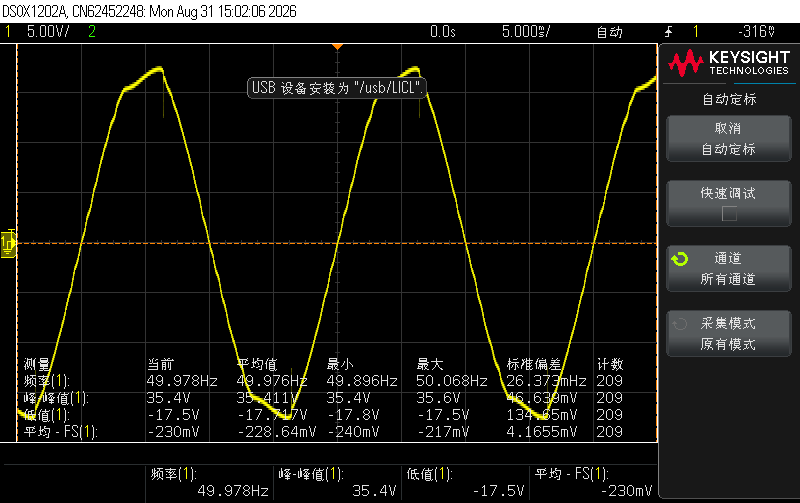
\includegraphics[width=0.9\linewidth]{data/断开A后断开A前49.assets/image-20260831155149384.png}
  \caption{断开 A 点后的输入侧波形}
  \label{fig:wave-open}
\end{figure}

\begin{figure}[p]
  \centering
  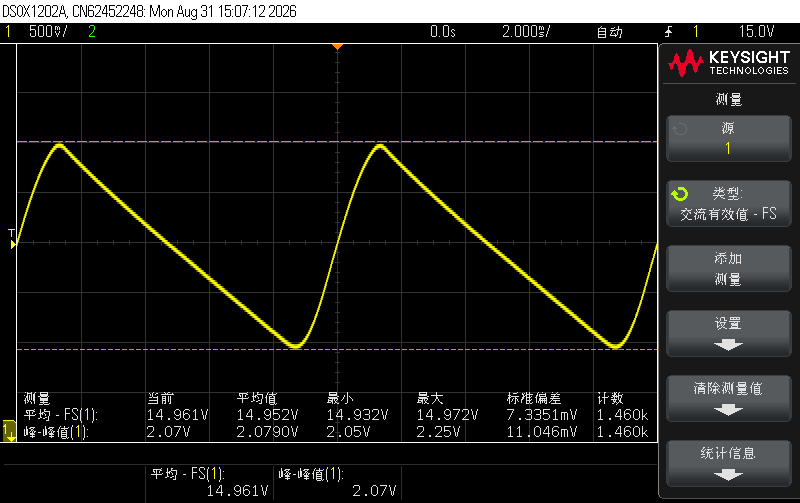
\includegraphics[width=0.9\linewidth]{data/断开A后断开A前49.assets/image-20260831155533057.png}
  \caption{接通 A 点后的输出侧波形}
  \label{fig:wave-connected}
\end{figure}

\begin{figure}[p]
  \centering
  \begin{tabular}{ccc}
    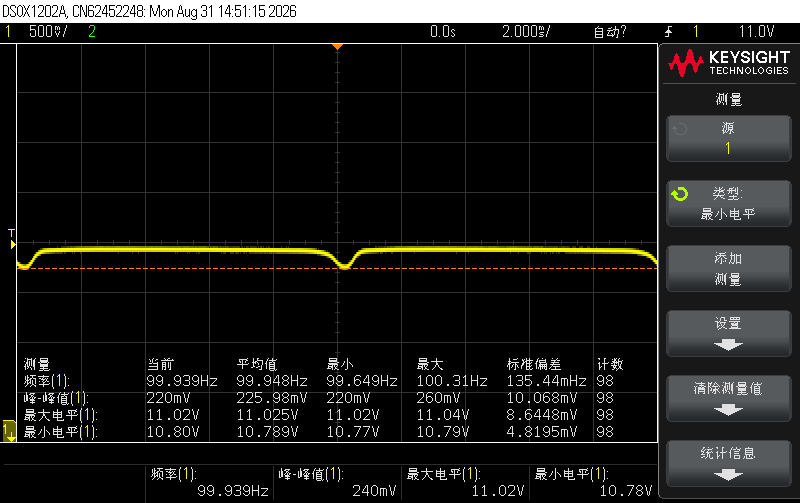
\includegraphics[width=0.29\linewidth]{data/pics/scope_4.png} &
    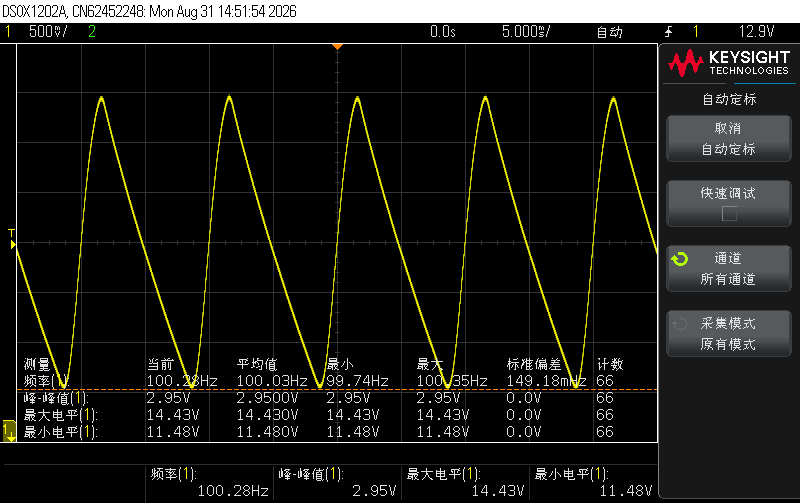
\includegraphics[width=0.29\linewidth]{data/pics/scope_6.png} &
    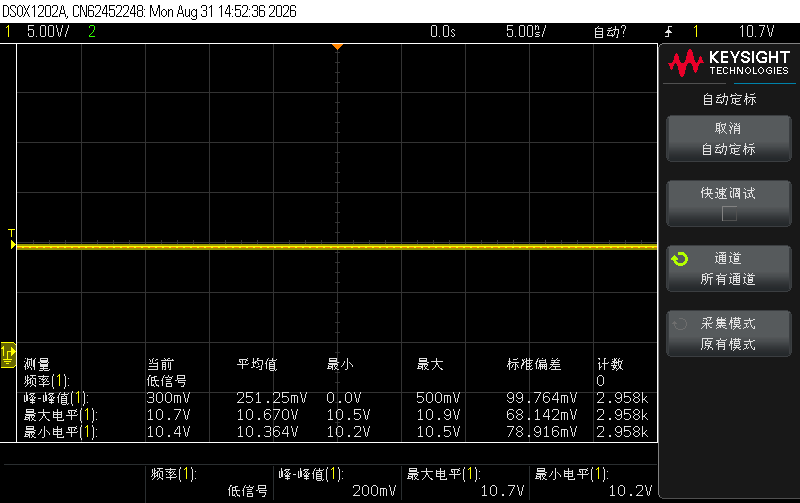
\includegraphics[width=0.29\linewidth]{data/pics/scope_7.png} \\
  \end{tabular}
  \caption{不同输出工作点下的波形对比（仅作定性展示）}
  \label{fig:wave-workpoints}
\end{figure}

\subsection{纹波抑制比}
表~\ref{table:ripple} 中输入纹波峰峰值为 $1.01\,\si{\volt}$，输出纹波峰峰值为 $6.37\,\si{\milli\volt}$。由式~\eqref{eq:ripple-rejection} 得
\[
  S_{S\mathrm{RPP}}=20\lg\frac{1.01}{6.37\times10^{-3}}
  =44.0\,\si{\decibel}.
\]
这里必须先将输出纹波的毫伏换算为伏。

将电压读数的最大允许误差按测量值的 $3\%$ 估计，并把误差区间视为均匀分布，则标准不确定度取为允许误差除以 $\sqrt{3}$。因此
\[
  u_i=\frac{0.03\times1.01}{\sqrt{3}}=0.0175\,\si{\volt},\qquad
  u_o=\frac{0.03\times6.37}{\sqrt{3}}=0.110\,\si{\milli\volt}.
\]
纹波抑制比的不确定度可由传播公式估计：
\[
  \delta S_{S\mathrm{RPP}}
  =\frac{20}{\ln 10}
   \sqrt{\left(\frac{u_i}{U_{i\mathrm{PP}}}\right)^2
       +\left(\frac{u_o}{U_{o\mathrm{PP}}}\right)^2}.
\]
代入数值得 $u_{S}=0.37\,\si{\decibel}$，取包含因子 $k=1.732$ 后的扩展不确定度为 $U_S=0.64\,\si{\decibel}$。因而纹波抑制比可表示为
\[
  S_{S\mathrm{RPP}}=(44.0\pm0.6)\,\si{\decibel}.
\]

\subsection{稳压系数与输出范围讨论}
由式~\eqref{eq:voltage-regulation}，稳压系数为
\[
  S_r=\frac{\Delta U_o/U_o}{\Delta U_i/U_i}.
\]
实验中应在负载电流和环境温度近似不变时，改变输入电压并记录对应的输出电压。本次数据只保留了输出电压的上下限，没有成对的 $U_i$ 读数，因而不能从本次测量独立求得 $S_r$ 。输出电压范围为
\[
  \Delta U_o=U_{o,\max}-U_{o,\min}=14.41-5.06=9.35\,\si{\volt},
\]
可用于衡量可调稳压电源的调节范围，但不等同于稳压系数。

\subsection{输出电阻}
取 $R_L=200\,\si{\ohm}$，由表~\ref{table:output-resistance} 的一次测量数据和式~\eqref{eq:output-resistance} 可得
\[
  R_o=\left(\frac{5.076}{5.071}-1\right)\times200
  =0.197\,\si{\ohm}.
\]
开路电压比负载电压高 $5\,\si{\milli\volt}$，得到的输出电阻为正值且较小，说明接入 $200\,\si{\ohm}$ 负载后输出电压只有较小下降。
从误差传播角度，若 $U'_o$ 、$U_o$ 和 $R_L$ 的标准不确定度分别为 $u_{U'}$ 、$u_U$ 和 $u_R$，则
\[
  u_{R_o}^2=\left(\frac{R_L}{U_o}\,u_{U'}\right)^2
  +\left(\frac{R_LU'_o}{U_o^2}\,u_U\right)^2
  +\left(\frac{U'_o}{U_o}-1\right)^2u_R^2.
\]
按与上述相同的 $3\%$ 电压相对误差估计，并取 $R_L$ 的相对误差为 $1\%$，有
\[
  u_{U'}=\frac{0.03\times5.076}{\sqrt{3}}=0.088\,\si{\volt},\quad
  u_U=\frac{0.03\times5.071}{\sqrt{3}}=0.088\,\si{\volt},\quad
  u_R=\frac{0.01\times200}{\sqrt{3}}=1.15\,\si{\ohm}.
\]
代入传播公式得合成标准不确定度 $u_{R_o}=4.91\,\si{\ohm}$，扩展不确定度为 $U_{R_o}=8.50\,\si{\ohm}$。按现有读数可写为
\[
  R_o=(0.2\pm8.5)\,\si{\ohm}\quad(k=1.732).
\]
由于开路与负载电压的差值仅为 $5\,\si{\milli\volt}$，按上述精度估计得到的不确定度远大于输出电阻本身。因此 $0.197\,\si{\ohm}$ 仅表示由当前读数得到的中心值，若要准确表征这一小输出电阻，需使用更高分辨率的电压测量或多次改变负载后进行拟合。

\section{实验的分析和总结}

实验中可调稳压电路的输出电压范围为 $5.06$--$14.41\,\si{\volt}$，说明调节电位器能够改变输出工作点。纹波测量得到输入纹波 $1.01\,\si{\volt}$、输出纹波 $6.37\,\si{\milli\volt}$，按定义计算的纹波抑制比约为 $44.0\,\si{\decibel}$，表明稳压器对交流纹波具有明显的抑制作用。

从工作原理看，7805 通过反馈调节串联调整元件，使取样电压与内部基准电压比较，并根据误差放大器的输出自动改变调整管的导通程度。输入电压经整流、滤波后仍含有周期性交流成分，滤波电容先减小其幅度，稳压器的反馈调节再进一步抑制纹波，所以输出纹波远小于输入纹波。波形图中约 $50\,\si{\hertz}$ 和约 $100\,\si{\hertz}$ 的频率读数与桥式整流的倍频特征基本一致，表明整流环节工作正常。

误差主要来自示波器和万用表的分辨率、波形峰峰值的自动测量算法、人工记录误差，以及整流电路输出随负载变化造成的工作点漂移。输出电阻由两个很接近的电压作差后计算，对万用表分辨率、导线接触电阻和电源波动尤其敏感。本次只进行一次负载测量，无法由重复数据评估 A 类不确定度。

按误差性质可将误差分为偶然误差和系统误差。偶然误差包括波形峰值判读的波动、万用表末位跳动和接线接触状态的短时变化，可通过多次测量取平均值来减小。系统误差包括万用表和示波器的固有精度限制、电阻电容的标称值偏差、电源频率和幅值波动，以及 7805 基准电压随温度漂移。实验时应先预热仪器，使探头与地线尽量短并保持接触稳固，同时在输出稳定后再读数。

输出电阻测量中，开路电压 $5.076\,\si{\volt}$ 略高于带负载电压 $5.071\,\si{\volt}$，变化方向符合电源内阻模型。但两者差值较小，重新测量时应在同一输入电压下先断开负载读取 $U'_o$，再接入已知 $R_L$ 读取 $U_o$，并增加重复测量次数。

接入 $200\,\si{\ohm}$ 负载后，负载电流和负载功率分别约为
\[
  I_L=\frac{5.071}{200}=25.36\,\si{\milli\ampere},\qquad
  P_L=U_oI_L=0.129\,\si{\watt}.
\]
从开路到带负载时，输出电压的相对下降为
\[
  \frac{U'_o-U_o}{U'_o}\times100\%=0.0985\%.
\]
这一结果表明，在本次负载条件下，输出电压的直流工作点变化很小。但由于所测电压差只有 $5\,\si{\milli\volt}$，这一结论主要适合作定性判断，输出电阻的高精度测量仍需更高分辨率的仪器和多组负载数据。

纹波电压幅值之比为
\[
  \frac{U_{i\mathrm{PP}}}{U_{o\mathrm{PP}}}
  =\frac{1.01}{6.37\times10^{-3}}\approx158.6.
\]
即输出纹波约为输入纹波的 $0.63\%$。该结果与 $44.0\,\si{\decibel}$ 的纹波抑制比相互印证，说明电容滤波和 7805 反馈稳压对整流后的交流分量起到了明显抑制作用。

\clearpage
\insertSignedDataPage

\end{document}
